%   ------------------------------------------------------------------------
\FloatBarrier
\section{Pixel Lab}
\label{s.pixelLabApendice}

\begin{figure}[htbp]
    \centering
    \caption{\small Tela de exportação no Pixel Lab}
    \label{fig:pixelLabExport}
    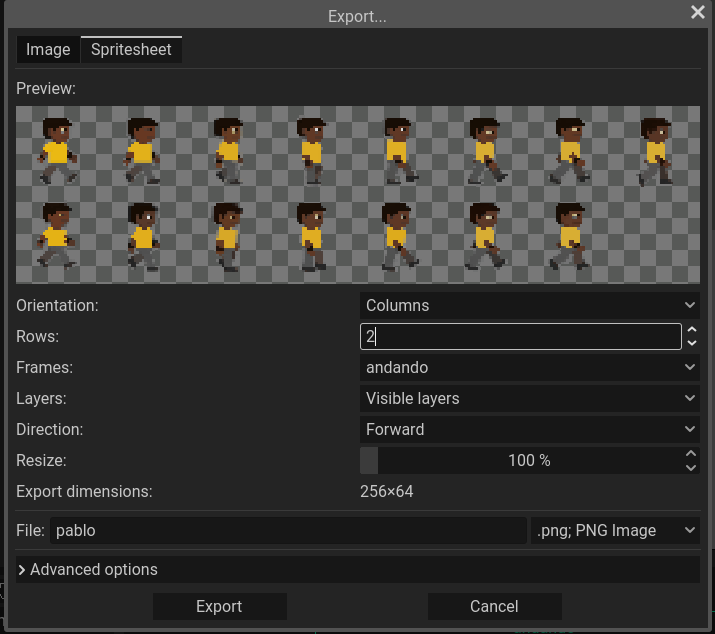
\includegraphics[width=0.7\linewidth]{figs/pixelLab/tela_exportar.PNG}
    \legend{\small Fonte: Elaborada pela autora.}
\end{figure}

\begin{figure}[htbp]
    \centering
    \caption{\small Funcionalidade para tocar a animação circulada em vermelho}
    \label{fig:pixelLabViewAnimation}
    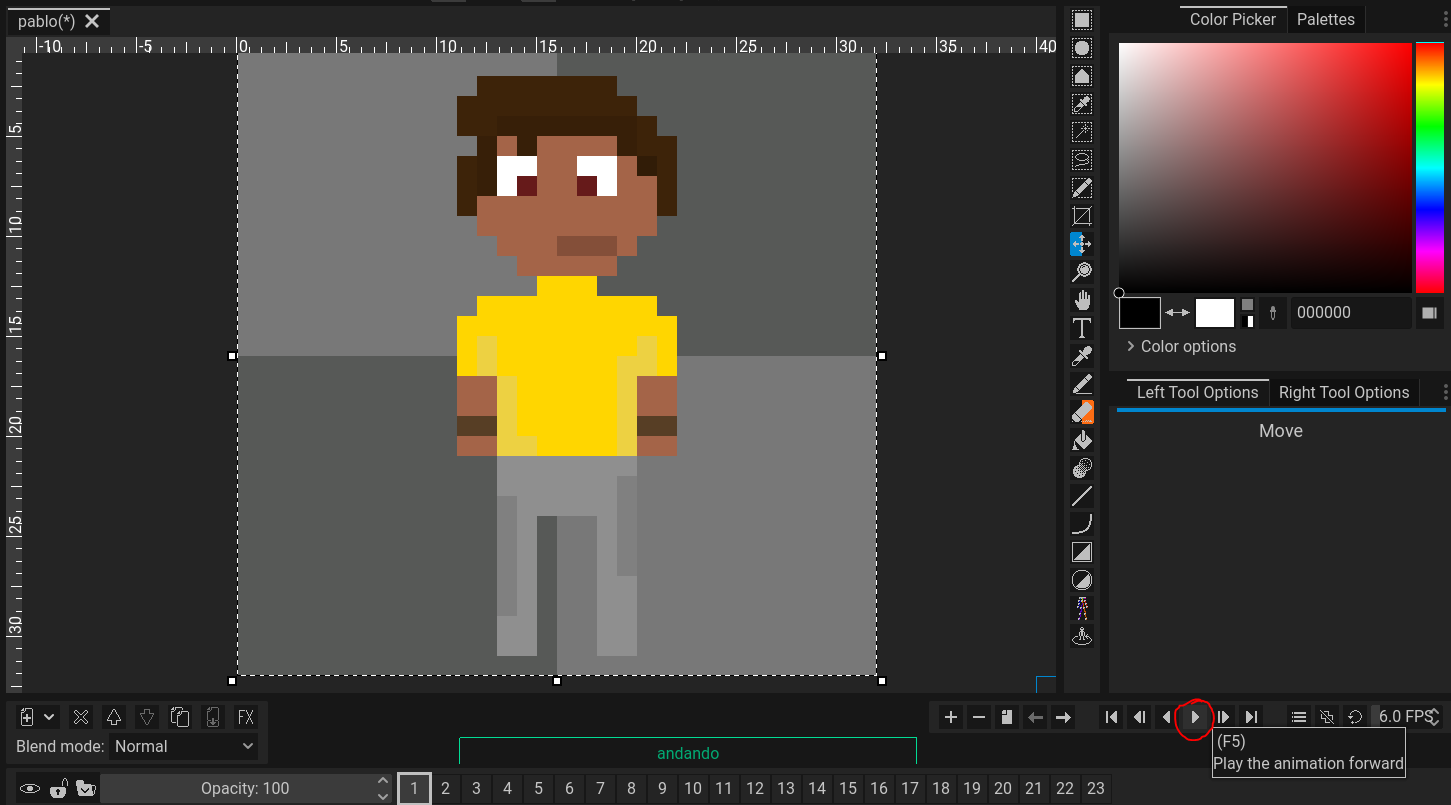
\includegraphics[width=0.7\linewidth]{figs/pixelLab/tela_ver_animacao.PNG}
    \legend{\small Fonte: Elaborada pela autora.}
\end{figure}

\begin{figure}[htbp]
    \centering
    \caption{\small Componente quick rotate circulado em vermelho}
    \label{fig:pixelLabQuickRotateTela}
    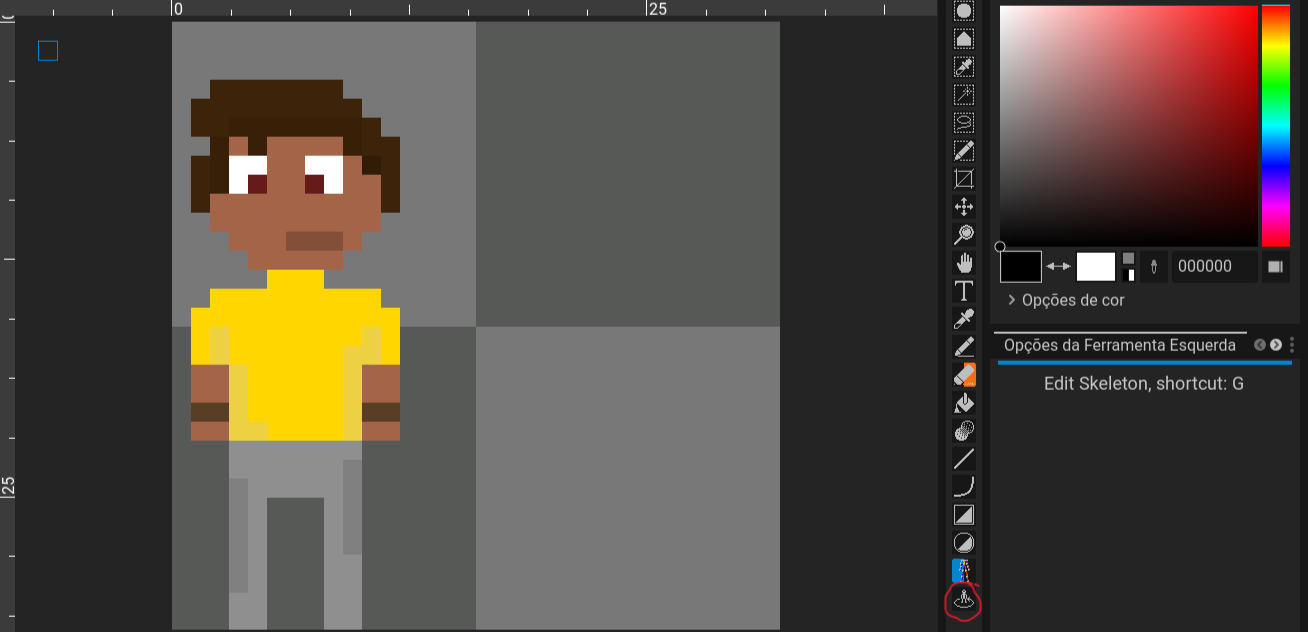
\includegraphics[width=0.7\linewidth]{figs/pixelLab/dia1/quick_rotate.PNG}
    \legend{\small Fonte: Elaborada pela autora.}
\end{figure}

\begin{figure}[htbp]
    \centering
    \caption{\small Tela Rotate no Pixel Lab}
    \label{fig:pixelLabRotateTela}
    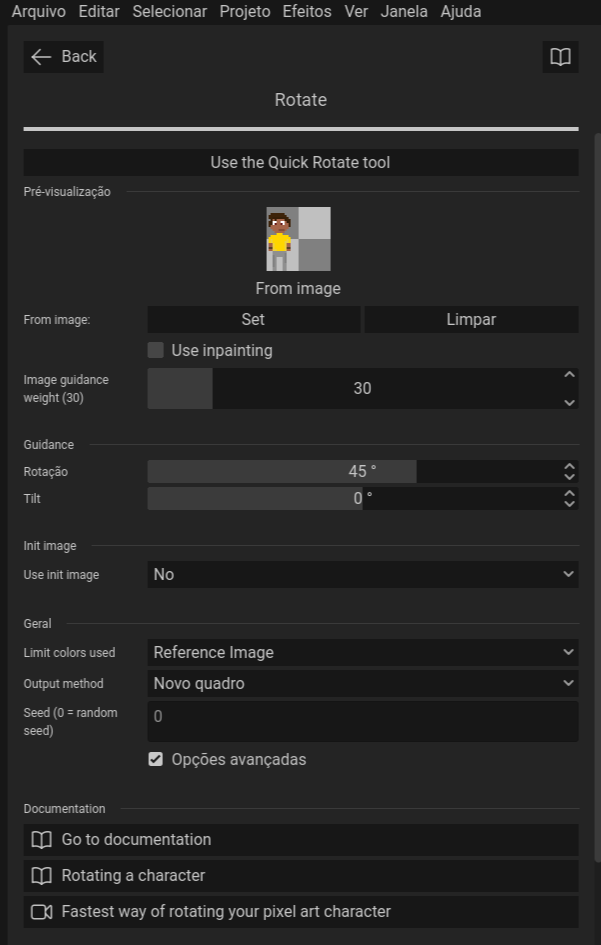
\includegraphics[width=0.4\linewidth]{figs/pixelLab/dia1/rotate.PNG}
    \legend{\small Fonte: Elaborada pela autora.}
\end{figure}

\begin{figure}[htbp]
    \centering
    \caption{\small Processo da utilização da ferramenta de rotação do PixelLab em junho/2025}
    \label{fig:pixelLabRotacao1}

    \begin{subfigure}{1\linewidth}
        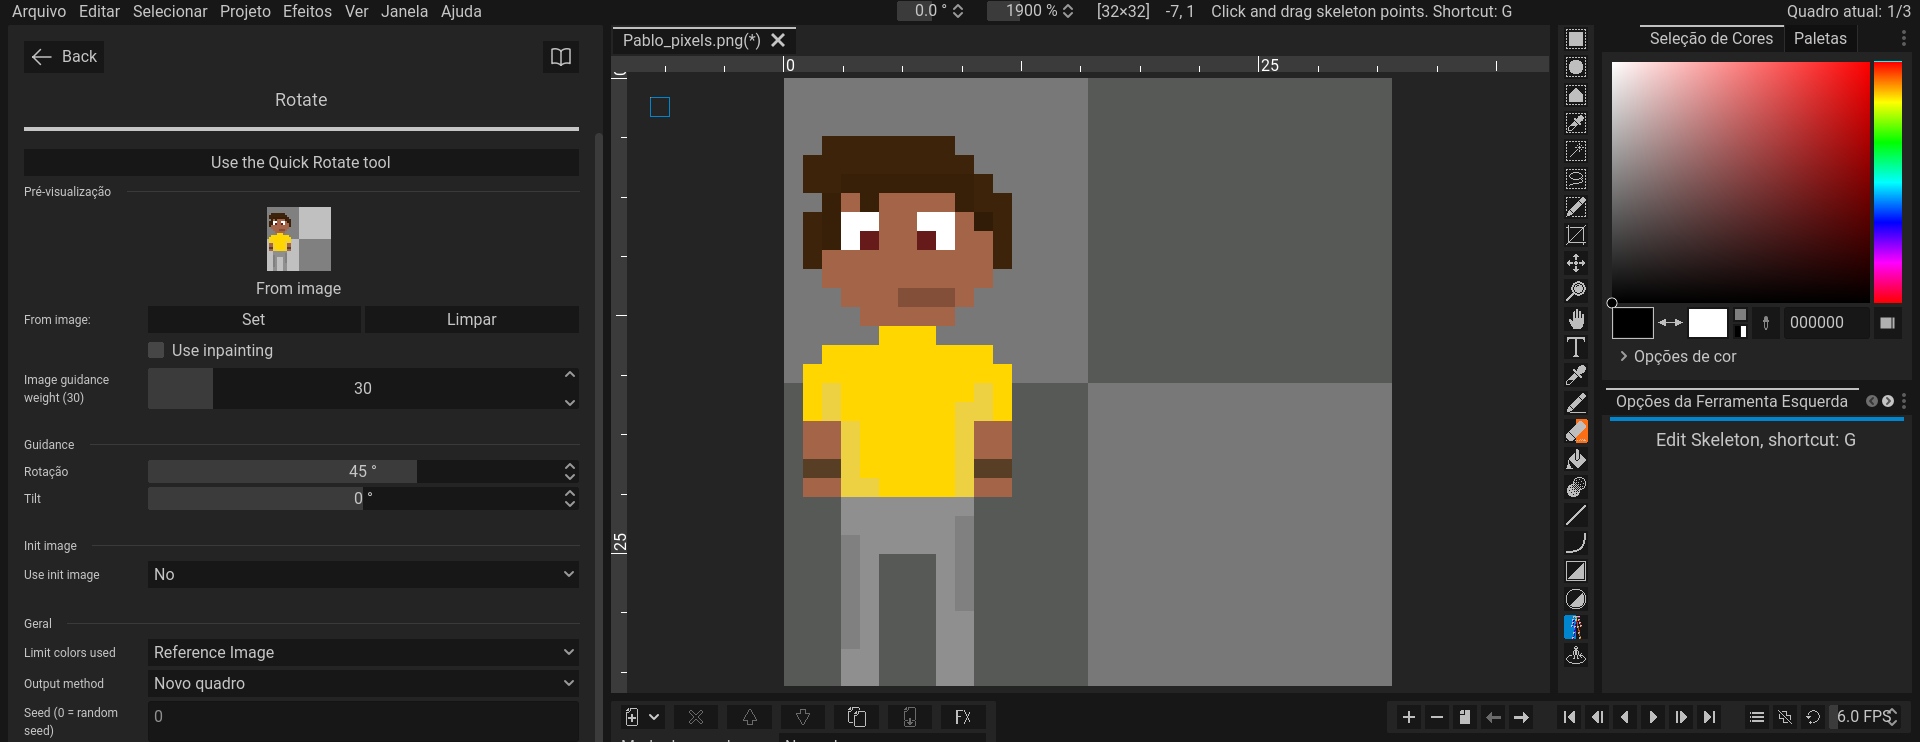
\includegraphics[width=1\linewidth]{figs/pixelLab/dia1/tela.PNG}
        \caption{\small Imagem que foi rotacionada}
        \label{fig:pixelLabRot1a}
    \end{subfigure}
    \begin{subfigure}{0.35\linewidth}
        
\includegraphics[width=1\linewidth]{figs/pixelLab/dia1/rotacao_1.PNG}
        \caption{\small Tentativa 1 de rotação de 90 graus.}
        \label{fig:pixelLabRot1b}
    \end{subfigure}
    \begin{subfigure}{0.35\linewidth}
        
\includegraphics[width=1\linewidth]{figs/pixelLab/dia1/resultado rotacao 2.PNG}
        \caption{\small Tentativa 2 de rotação de 90 graus.}
        \label{fig:pixelLabRot1c}
    \end{subfigure}
    \begin{subfigure}{0.35\linewidth}
        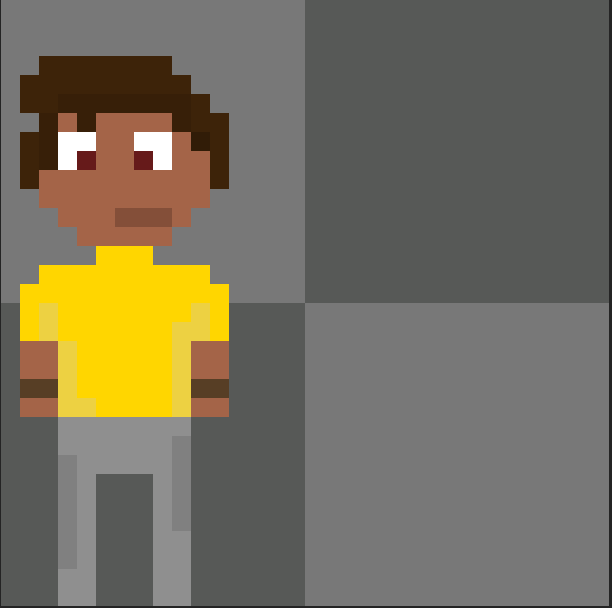
\includegraphics[width=1\linewidth]{figs/pixelLab/dia1/rotacao 90 graus.PNG}
        \caption{\small Tentativa de rotação de 90 graus com o quick rotate.}
        \label{fig:pixelLabRot1d}
    \end{subfigure}

    
    \legend{\small Fonte: Elaborada pela autora, utilizando a ferramenta Pixel Lab.}
\end{figure}

\begin{figure}[htbp]
    \centering
    \caption{\small Processo da utilização 1 da ferramenta de rotação do PixelLab em julho/2025}
    \label{fig:pixelLabRotacao2}

    \begin{subfigure}{0.32\linewidth}
        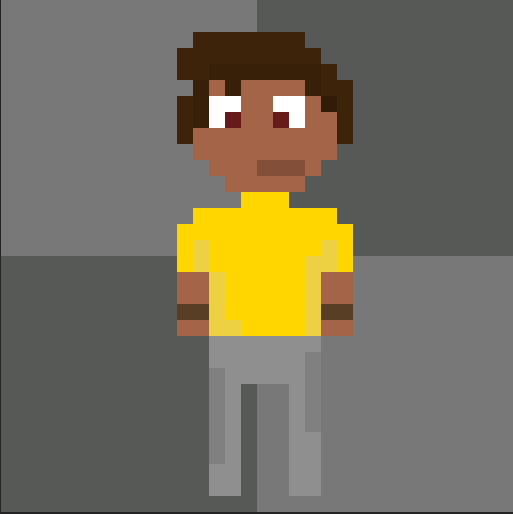
\includegraphics[width=1\linewidth]{figs/pixelLab/dia2/sprite_centro.PNG}
        \caption{\small Imagem que foi rotacionada}
        \label{fig:pixelLabRot2a}
    \end{subfigure}
    \begin{subfigure}{0.32\linewidth}
        
\includegraphics[width=1\linewidth]{figs/pixelLab/dia2/rot90res1.PNG}
        \caption{\small Tentativa 1 de rotação de 90 graus}
        \label{fig:pixelLabRot2b}
    \end{subfigure}
    \begin{subfigure}{0.32\linewidth}
        
\includegraphics[width=1\linewidth]{figs/pixelLab/dia2/rot90res2.PNG}
        \caption{\small Tentativa 2 de rotação de 90 graus}
        \label{fig:pixelLabRot2c}
    \end{subfigure}
    \legend{\small Fonte: Elaborada pela autora, utilizando a ferramenta Pixel Lab.}
\end{figure}

\begin{figure}[htbp]
    \centering
    \caption{\small Processo da utilização 2 da ferramenta de rotação do PixelLab em julho/2025}
    \label{fig:pixelLabRotacao3}

    \begin{subfigure}{0.32\linewidth}
        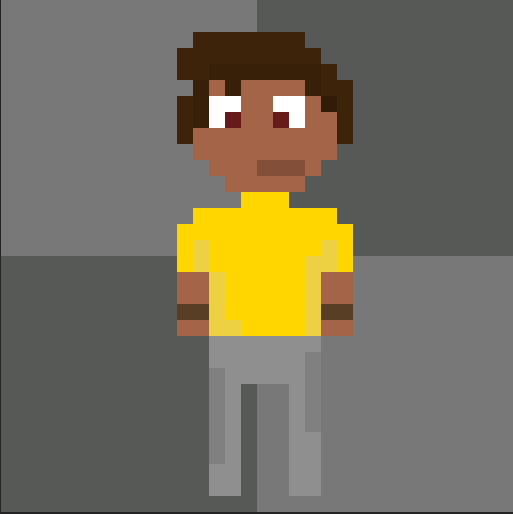
\includegraphics[width=1\linewidth]{figs/pixelLab/dia2/sprite_centro.PNG}
        \caption{\small Imagem que foi rotacionada}
        \label{fig:pixelLabRot3a}
    \end{subfigure}
    \begin{subfigure}{0.32\linewidth}
        
\includegraphics[width=1\linewidth]{figs/pixelLab/dia2/rot45res3.PNG}
        \caption{\small Rotação de 45 graus}
        \label{fig:pixelLabRot3b}
    \end{subfigure}
    \begin{subfigure}{0.32\linewidth}
        
\includegraphics[width=1\linewidth]{figs/pixelLab/dia2/rot90res3.PNG}
        \caption{\small Rotação de 90 graus a partir do resultado da rotação de 45 graus}
        \label{fig:pixelLabRot3c}
    \end{subfigure}
    \legend{\small Fonte: Elaborada pela autora, utilizando a ferramenta Pixel Lab.}
\end{figure}

\begin{figure}[htbp]
    \centering
    \caption{\small Processo da utilização 3 da ferramenta de rotação do PixelLab em julho/2025}
    \label{fig:pixelLabRotacao4}

    \begin{subfigure}{0.32\linewidth}
        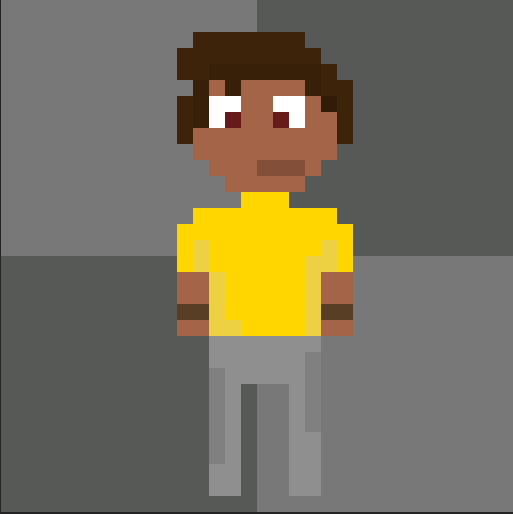
\includegraphics[width=1\linewidth]{figs/pixelLab/dia2/sprite_centro.PNG}
        \caption{\small Imagem que foi rotacionada}
        \label{fig:pixelLabRot4a}
    \end{subfigure}
    \begin{subfigure}{0.32\linewidth}
        
\includegraphics[width=1\linewidth]{figs/pixelLab/dia2/rot45res4.PNG}
        \caption{\small Rotação de 45 graus}
        \label{fig:pixelLabRot4b}
    \end{subfigure}
    \begin{subfigure}{0.32\linewidth}
        
\includegraphics[width=1\linewidth]{figs/pixelLab/dia2/rot90res4.PNG}
        \caption{\small Rotação de 90 graus a partir do resultado da rotação de 45 graus}
        \label{fig:pixelLabRot4c}
    \end{subfigure}
    \legend{\small Fonte: Elaborada pela autora, utilizando a ferramenta Pixel Lab.}
\end{figure}


\begin{figure}[htbp]
    \centering
    \caption{\small Processo da utilização 4 da ferramenta de rotação do PixelLab em julho/2025}
    \label{fig:pixelLabRotacao5}

    \begin{subfigure}{0.32\linewidth}
        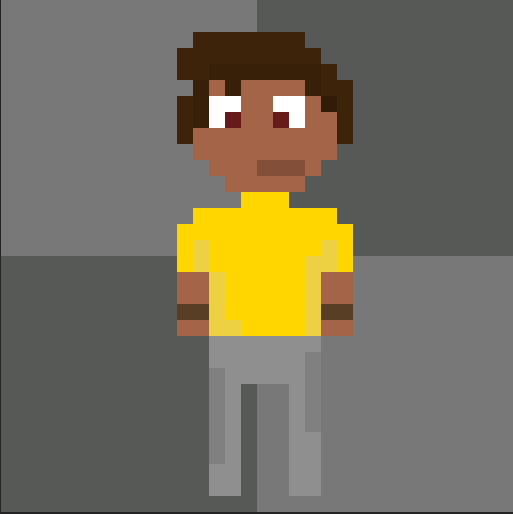
\includegraphics[width=1\linewidth]{figs/pixelLab/dia2/sprite_centro.PNG}
        \caption{\small Imagem que foi rotacionada}
        \label{fig:pixelLabRot5a}
    \end{subfigure}
    \begin{subfigure}{0.32\linewidth}
        
\includegraphics[width=1\linewidth]{figs/pixelLab/dia2/rotacao 45 graus quick rotate.PNG}
        \caption{\small Rotação rápida de 45 graus}
        \label{fig:pixelLabRot5b}
    \end{subfigure}
    \begin{subfigure}{0.32\linewidth}
        
\includegraphics[width=1\linewidth]{figs/pixelLab/dia2/rotacao 90 graus quick rotate.PNG}
        \caption{\small Rotação rápida de 90 graus}
        \label{fig:pixelLabRot5c}
    \end{subfigure}
    \legend{\small Fonte: Elaborada pela autora, utilizando a ferramenta Pixel Lab.}
\end{figure}

\begin{figure}[htbp]
    \centering
    \caption{\small Ajuste fino nos resultados da rotação de 45 graus}
    \label{fig:pixelLabAjusteFino2}
    \begin{subfigure}{0.32\linewidth}
        \centering
        
\includegraphics[width=1\linewidth]{figs/pixelLab/dia2/rot45res3.PNG}
        \caption{\small Corpo a ser utilizado para edição}
        \label{fig:pixelLabAjusteFino2a}
    \end{subfigure}
    \begin{subfigure}{0.32\linewidth}
        \centering
        
\includegraphics[width=1\linewidth]{figs/pixelLab/dia2/rot45res4.PNG}
        \caption{\small Cabeça a ser utilizada para edição}
        \label{fig:pixelLabAjusteFino2b}
    \end{subfigure}
    \begin{subfigure}{0.32\linewidth}
        \centering
        
\includegraphics[width=0.83\linewidth]{figs/pixelLab/dia2/fix_teste_3.PNG}
        \caption{\small Após edição}
        \label{fig:pixelLabAjusteFino2c}
    \end{subfigure}

    \legend{\small Fonte: Elaborada pela autora, utilizando a ferramenta Pixel Lab.}
\end{figure}

\begin{figure}[htbp]
    \centering
    \caption{\small Processo da utilização 5 da ferramenta de rotação do PixelLab em julho/2025}
    \label{fig:pixelLabRotacao6}

    \begin{subfigure}{0.32\linewidth}
        
\includegraphics[width=1\linewidth]{figs/pixelLab/dia2/fix_teste_4.PNG}
        \caption{\small Imagem que foi rotacionada}
        \label{fig:pixelLabRot6a}
    \end{subfigure}
    \begin{subfigure}{0.32\linewidth}
        
\includegraphics[width=1\linewidth]{figs/pixelLab/dia2/rot45fix4res1.PNG}
        \caption{\small Tentativa 1 de rotação de 90 graus}
        \label{fig:pixelLabRot6b}
    \end{subfigure}
    \begin{subfigure}{0.32\linewidth}
        
\includegraphics[width=1\linewidth]{figs/pixelLab/dia2/rot45fix4res2.PNG}
        \caption{\small Tentativa 2 de rotação de 90 graus}
        \label{fig:pixelLabRot6c}
    \end{subfigure}
    \legend{\small Fonte: Elaborada pela autora, utilizando a ferramenta Pixel Lab.}
\end{figure}

\begin{figure}[htbp]
    \centering
    \caption{\small Processo da utilização 6 da ferramenta de rotação do PixelLab em julho/2025}
    \label{fig:pixelLabRotacao7}

    \begin{subfigure}{0.45\linewidth}
        
\includegraphics[width=1\linewidth]{figs/pixelLab/dia2/fix_teste_4.PNG}
        \caption{\small Imagem que foi rotacionada}
        \label{fig:pixelLabRot7a}
    \end{subfigure}
    \begin{subfigure}{0.45\linewidth}
        
\includegraphics[width=1\linewidth]{figs/pixelLab/dia2/rotacao 45 graus fix4 quick rotate.PNG}
        \caption{\small Rotação rápida de 90 graus}
        \label{fig:pixelLabRot7b}
    \end{subfigure}
    \legend{\small Fonte: Elaborada pela autora, utilizando a ferramenta Pixel Lab.}
\end{figure}

\begin{figure}[htbp]
    \centering
    \caption{\small Processo da utilização 7 da ferramenta de rotação do PixelLab em julho/2025}
    \label{fig:pixelLabRotacao8}

    \begin{subfigure}{0.35\linewidth}
        
\includegraphics[width=0.83\linewidth]{figs/pixelLab/dia2/fix_teste_3.PNG}
        \caption{\small Imagem que foi rotacionada}
        \label{fig:pixelLabRot8a}
    \end{subfigure}
    \begin{subfigure}{0.35\linewidth}
        
\includegraphics[width=1\linewidth]{figs/pixelLab/dia2/rot45fix3res1.PNG}
        \caption{\small Tentativa 1 de rotação de 90 graus}
        \label{fig:pixelLabRot8b}
    \end{subfigure}
    \begin{subfigure}{0.35\linewidth}
        
\includegraphics[width=1\linewidth]{figs/pixelLab/dia2/rot45fix3res2.PNG}
        \caption{\small Tentativa 2 de rotação de 90 graus}
        \label{fig:pixelLabRot8c}
    \end{subfigure}
    \begin{subfigure}{0.35\linewidth}
        
\includegraphics[width=1\linewidth]{figs/pixelLab/dia2/rot45fix3res3.PNG}
        \caption{\small Tentativa 3 de rotação de 90 graus}
        \label{fig:pixelLabRot8d}
    \end{subfigure}
    \legend{\small Fonte: Elaborada pela autora, utilizando a ferramenta Pixel Lab.}
\end{figure}


\begin{figure}[htbp]
    \centering
    \caption{\small Processo da utilização 8 da ferramenta de rotação do PixelLab em julho/2025}
    \label{fig:pixelLabRotacao9}

    \begin{subfigure}{0.35\linewidth}
        
\includegraphics[width=1\linewidth]{figs/pixelLab/dia2/fix_teste_3.PNG}
        \caption{\small Imagem que foi rotacionada}
        \label{fig:pixelLabRot9a}
    \end{subfigure}
    \begin{subfigure}{0.35\linewidth}
        
\includegraphics[width=0.83\linewidth]{figs/pixelLab/dia2/rotacao 45 graus fix3 quick rotate.PNG}
        \caption{\small Rotação rápida de 90 graus}
        \label{fig:pixelLabRot9b}
    \end{subfigure}
    \legend{\small Fonte: Elaborada pela autora, utilizando a ferramenta Pixel Lab.}
\end{figure}

\begin{figure}[htbp]
    \centering
    \caption{\small Tela Rotate com o melhor resultado como imagem de inicialização no Pixel Lab}
    \label{fig:pixelLabRotInit}
    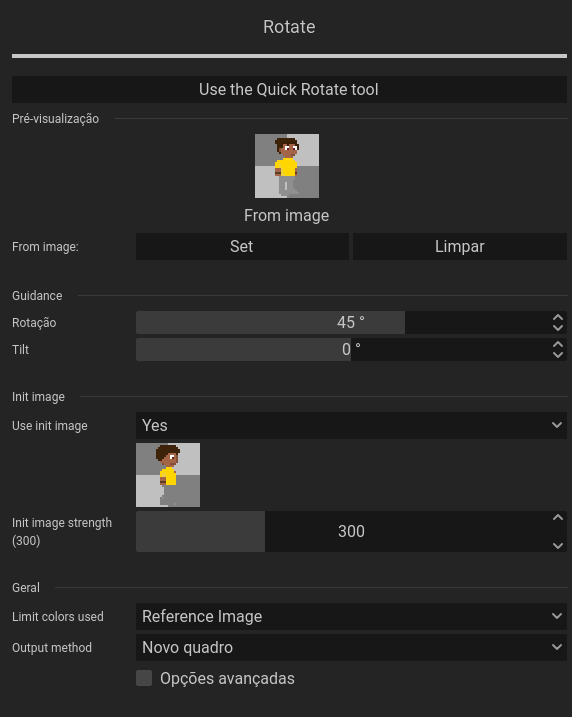
\includegraphics[width=0.7\linewidth]{figs/pixelLab/dia2/menu_fix3_init1.PNG}
    \legend{\small Fonte: Elaborada pela autora.}
\end{figure}

\begin{figure}[htbp]
    \centering
    \caption{\small Processo da utilização 9 da ferramenta de rotação do PixelLab em julho/2025}
    \label{fig:pixelLabRotacao10}

    \begin{subfigure}{0.24\linewidth}
        
\includegraphics[width=0.83\linewidth]{figs/pixelLab/dia2/fix_teste_3.PNG}
        \caption{\small Imagem que foi rotacionada}
        \label{fig:pixelLabRotacao10a}
    \end{subfigure}
    \begin{subfigure}{0.24\linewidth}
        
\includegraphics[width=1\linewidth]{figs/pixelLab/dia2/init.PNG}
        \caption{\small Imagem usada de inicialização com init image strength em 300}
        \label{fig:pixelLabRotacao10b}
    \end{subfigure}
    \begin{subfigure}{0.24\linewidth}
        
\includegraphics[width=1\linewidth]{figs/pixelLab/dia2/rot45fix3init1res1.PNG}
        \caption{\small Tentativa 1 de rotação de 90 graus}
        \label{fig:pixelLabRotacao10c}
    \end{subfigure}
    \begin{subfigure}{0.24\linewidth}
        
\includegraphics[width=1\linewidth]{figs/pixelLab/dia2/rot45fix3init1res2.PNG}
        \caption{\small Tentativa 2 de rotação de 90 graus}
        \label{fig:pixelLabRotacao10d}
    \end{subfigure}
    \legend{\small Fonte: Elaborada pela autora, utilizando a ferramenta Pixel Lab.}
\end{figure}

\begin{figure}[htbp]
    \centering
    \caption{\small Processo da utilização 9 da ferramenta de rotação do PixelLab em julho/2025}
    \label{fig:pixelLabRotacao11}

    \begin{subfigure}{0.32\linewidth}
        
\includegraphics[width=0.83\linewidth]{figs/pixelLab/dia2/fix_teste_3.PNG}
        \caption{\small Imagem que foi rotacionada}
        \label{fig:pixelLabRotacao11a}
    \end{subfigure}
    \begin{subfigure}{0.32\linewidth}
        
\includegraphics[width=1\linewidth]{figs/pixelLab/dia2/fix_init_1.PNG}
        \caption{\small Imagem usada de inicialização}
        \label{fig:pixelLabRotacao11b}
    \end{subfigure}
    \begin{subfigure}{0.32\linewidth}
        
\includegraphics[width=1\linewidth]{figs/pixelLab/dia2/rot45fix3init1res3.PNG}
        \caption{\small Rotação de 90 graus com init image strength em 300}
        \label{fig:pixelLabRotacao11c}
    \end{subfigure}
    \begin{subfigure}{0.32\linewidth}
        
\includegraphics[width=1\linewidth]{figs/pixelLab/dia2/rot45fix3init1res4.PNG}
        \caption{\small Rotação de 90 graus com init image strength em 600}
        \label{fig:pixelLabRotacao11d}
    \end{subfigure}
    \begin{subfigure}{0.32\linewidth}
        
\includegraphics[width=1\linewidth]{figs/pixelLab/dia2/rot45fix3init1res5.PNG}
        \caption{\small Rotação de 90 graus com init image strength em 180}
        \label{fig:pixelLabRotacao11e}
    \end{subfigure}
    \legend{\small Fonte: Elaborada pela autora, utilizando a ferramenta Pixel Lab.}
\end{figure}


\begin{figure}[htbp]
    \centering
    \caption{\small Processo da utilização 1 da ferramenta de animação do PixelLab em julho/2025}
    \label{fig:pixelLabAnimacao1}

    \begin{subfigure}{0.6\linewidth}
        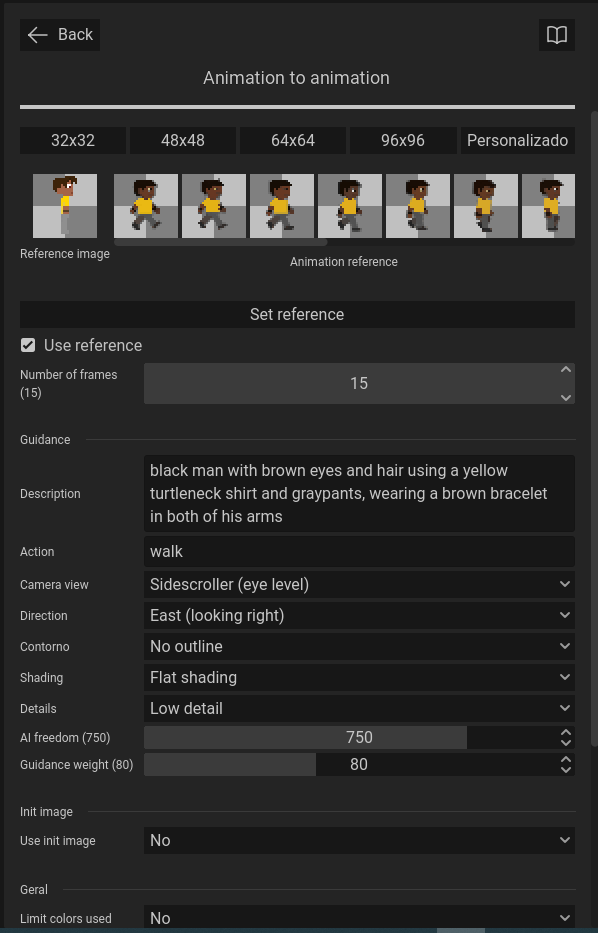
\includegraphics[width=1\linewidth]{figs/pixelLab/dia3/tela_2.PNG}
        \caption{\small Configurações da geração de animação}
        \label{fig:pixelLabAnimacao1a}
    \end{subfigure}
    \begin{subfigure}{0.35\linewidth}
        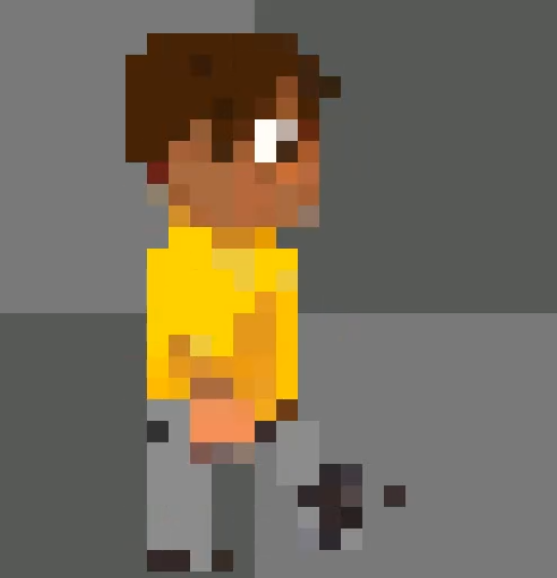
\includegraphics[width=1\linewidth]{figs/pixelLab/dia3/print2.PNG}
        \caption{\small Frame da animação gerada}
        \label{fig:pixelLabAnimacao1b}
    \end{subfigure}
    \legend{\small Fonte: Elaborada pela autora, utilizando a ferramenta Pixel Lab.}
\end{figure}

\begin{figure}[htbp]
    \centering
    \caption{\small Processo da utilização 2 da ferramenta de animação do PixelLab em julho/2025}
    \label{fig:pixelLabAnimacao2}

    \begin{subfigure}{0.6\linewidth}
        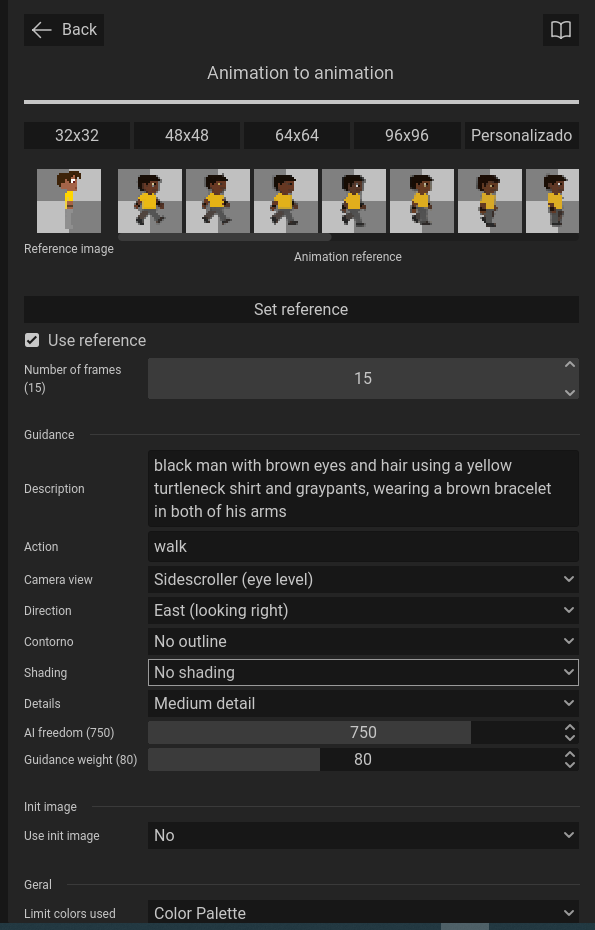
\includegraphics[width=1\linewidth]{figs/pixelLab/dia3/tela_3.PNG}
        \caption{\small Configurações da geração de animação}
        \label{fig:pixelLabAnimacao2a}
    \end{subfigure}
    \begin{subfigure}{0.35\linewidth}
        
\includegraphics[width=1\linewidth]{figs/pixelLab/dia3/print3.PNG}
        \caption{\small Frame da animação gerada}
        \label{fig:pixelLabAnimacao2b}
    \end{subfigure}
    \legend{\small Fonte: Elaborada pela autora, utilizando a ferramenta Pixel Lab.}
\end{figure}

\begin{figure}[htbp]
    \centering
    \caption{\small Processo da utilização 3 da ferramenta de animação do PixelLab em julho/2025}
    \label{fig:pixelLabAnimacao3}

    \begin{subfigure}{0.6\linewidth}
        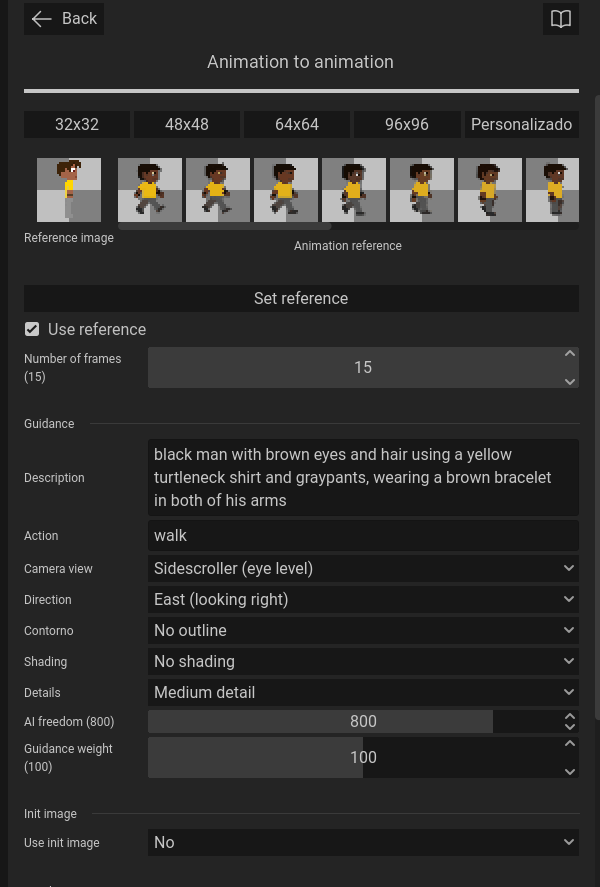
\includegraphics[width=1\linewidth]{figs/pixelLab/dia3/tela_4.PNG}
        \caption{\small Configurações da geração de animação}
        \label{fig:pixelLabAnimacao3a}
    \end{subfigure}
    \begin{subfigure}{0.35\linewidth}
        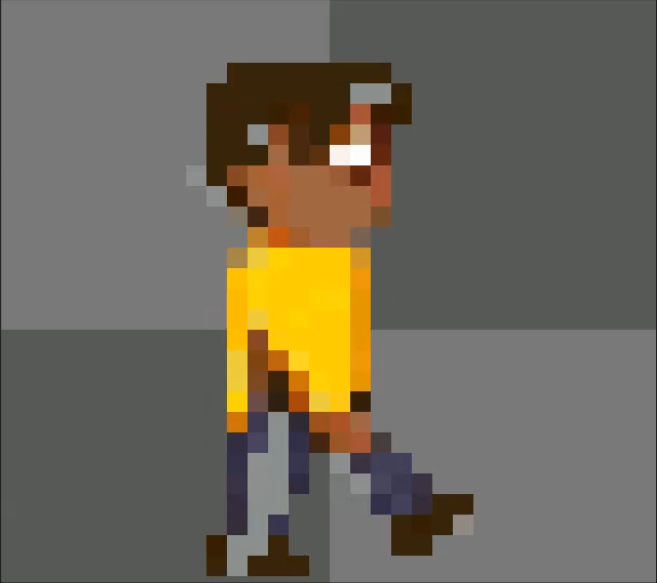
\includegraphics[width=1\linewidth]{figs/pixelLab/dia3/print4.PNG}
        \caption{\small Frame da animação gerada}
        \label{fig:pixelLabAnimacao3b}
    \end{subfigure}
    \legend{\small Fonte: Elaborada pela autora, utilizando a ferramenta Pixel Lab.}
\end{figure}

\begin{figure}[htbp]
    \centering
    \caption{\small Processo da utilização 4 da ferramenta de animação do PixelLab em julho/2025}
    \label{fig:pixelLabAnimacao4}

    \begin{subfigure}{0.6\linewidth}
        \includegraphics[width=1\linewidth]{figs/pixelLab/dia3/tela_5.PNG}
        \caption{\small Configurações da geração de animação}
        \label{fig:pixelLabAnimacao4a}
    \end{subfigure}
    \begin{subfigure}{0.35\linewidth}
        \includegraphics[width=1\linewidth]{figs/pixelLab/dia3/print5.PNG}
        \caption{\small Frame da animação gerada}
        \label{fig:pixelLabAnimacao4b}
    \end{subfigure}
    \legend{\small Fonte: Elaborada pela autora, utilizando a ferramenta Pixel Lab.}
\end{figure}

\begin{figure}[htbp]
    \centering
    \caption{\small Processo da utilização 5 da ferramenta de animação do PixelLab em julho/2025}
    \label{fig:pixelLabAnimacao5}

    \begin{subfigure}{0.6\linewidth}
        \includegraphics[width=1\linewidth]{figs/pixelLab/dia3/tela_6.PNG}
        \caption{\small Configurações da geração de animação}
        \label{fig:pixelLabAnimacao5a}
    \end{subfigure}
    \begin{subfigure}{0.35\linewidth}
        \includegraphics[width=1\linewidth]{figs/pixelLab/dia3/print6.PNG}
        \caption{\small Frame da animação gerada}
        \label{fig:pixelLabAnimacao5b}
    \end{subfigure}
    \legend{\small Fonte: Elaborada pela autora, utilizando a ferramenta Pixel Lab.}
\end{figure}

\begin{figure}[htbp]
    \centering
    \caption{\small Processo da utilização 6 da ferramenta de animação do PixelLab em julho/2025}
    \label{fig:pixelLabAnimacao6}

    \begin{subfigure}{0.6\linewidth}
        \includegraphics[width=1\linewidth]{figs/pixelLab/dia3/tela_7.PNG}
        \caption{\small Configurações da geração de animação}
        \label{fig:pixelLabAnimacao6a}
    \end{subfigure}
    \begin{subfigure}{0.35\linewidth}
        \includegraphics[width=1\linewidth]{figs/pixelLab/dia3/print7.PNG}
        \caption{\small Frame da animação gerada}
        \label{fig:pixelLabAnimacao6b}
    \end{subfigure}
    \legend{\small Fonte: Elaborada pela autora, utilizando a ferramenta Pixel Lab.}
\end{figure}

\begin{figure}[htbp]
    \centering
    \caption{\small Processo da utilização 7 da ferramenta de animação do PixelLab em julho/2025}
    \label{fig:pixelLabAnimacao7}

    \begin{subfigure}{0.6\linewidth}
        \includegraphics[width=1\linewidth]{figs/pixelLab/dia4/tela1.PNG}
        \caption{\small Configurações da geração de animação}
        \label{fig:pixelLabAnimacao7a}
    \end{subfigure}
    \begin{subfigure}{0.35\linewidth}
        \includegraphics[width=1\linewidth]{figs/pixelLab/dia4/print1.PNG}
        \caption{\small Frame da animação gerada}
        \label{fig:pixelLabAnimacao7b}
    \end{subfigure}
    \legend{\small Fonte: Elaborada pela autora, utilizando a ferramenta Pixel Lab.}
\end{figure}

\begin{figure}[htbp]
    \centering
    \caption{\small Processo da utilização 8 da ferramenta de animação do PixelLab em julho/2025}
    \label{fig:pixelLabAnimacao8}

    \begin{subfigure}{0.6\linewidth}
        \includegraphics[width=1\linewidth]{figs/pixelLab/dia4/tela2.PNG}
        \caption{\small Configurações da geração de animação}
        \label{fig:pixelLabAnimacao8a}
    \end{subfigure}
    \begin{subfigure}{0.35\linewidth}
        \includegraphics[width=1\linewidth]{figs/pixelLab/dia4/print2.PNG}
        \caption{\small Frame da animação gerada}
        \label{fig:pixelLabAnimacao8b}
    \end{subfigure}
    \legend{\small Fonte: Elaborada pela autora, utilizando a ferramenta Pixel Lab.}
\end{figure}

\begin{figure}[htbp]
    \centering
    \caption{\small Processo da utilização 9 da ferramenta de animação do PixelLab em julho/2025}
    \label{fig:pixelLabAnimacao9}

    \begin{subfigure}{0.6\linewidth}
        \includegraphics[width=1\linewidth]{figs/pixelLab/dia4/tela4_animarLimitando as cores.PNG}
        \caption{\small Configurações da geração de animação}
        \label{fig:pixelLabAnimacao9a}
    \end{subfigure}
    \begin{subfigure}{0.35\linewidth}
        \includegraphics[width=1\linewidth]{figs/pixelLab/dia4/print4.PNG}
        \caption{\small Frame da animação gerada}
        \label{fig:pixelLabAnimacao9b}
    \end{subfigure}
    \legend{\small Fonte: Elaborada pela autora, utilizando a ferramenta Pixel Lab.}
\end{figure}

\begin{figure}[htbp]
    \centering
    \caption{\small Processo da utilização 10 da ferramenta de animação do PixelLab em julho/2025}
    \label{fig:pixelLabAnimacao10}

    \begin{subfigure}{0.6\linewidth}
        \includegraphics[width=1\linewidth]{figs/pixelLab/dia4/tela5_teste2.PNG}
        \caption{\small Configurações da geração de animação}
        \label{fig:pixelLabAnimacao10a}
    \end{subfigure}
    \begin{subfigure}{0.35\linewidth}
        \includegraphics[width=1\linewidth]{figs/pixelLab/dia4/print5.PNG}
        \caption{\small Frame da animação gerada}
        \label{fig:pixelLabAnimacao10b}
    \end{subfigure}
    \legend{\small Fonte: Elaborada pela autora, utilizando a ferramenta Pixel Lab.}
\end{figure}

\begin{figure}[htbp]
    \centering
    \caption{\small Processo da utilização 11 da ferramenta de animação do PixelLab em julho/2025}
    \label{fig:pixelLabAnimacao11}

    \begin{subfigure}{0.6\linewidth}
        \includegraphics[width=1\linewidth]{figs/pixelLab/dia4/tela6.PNG}
        \caption{\small Configurações da geração de animação}
        \label{fig:pixelLabAnimacao11a}
    \end{subfigure}
    \begin{subfigure}{0.35\linewidth}
        \includegraphics[width=1\linewidth]{figs/pixelLab/dia4/print6.PNG}
        \caption{\small Frame da animação gerada}
        \label{fig:pixelLabAnimacao11b}
    \end{subfigure}
    \legend{\small Fonte: Elaborada pela autora, utilizando a ferramenta Pixel Lab.}
\end{figure}